% Chapter 5

\chapter{Discussion} % Main chapter title

\label{Chapter5} % For referencing the chapter elsewhere, use \ref{Chapter5}

%----------------------------------------------------------------------------------------

This chapter interprets the results of Chapter~\ref{Chapter4}: it answers the research questions, attributes the improvement to its source, explains why learning the destruction size did not help, compares the outcome with the expectations of the design brief and states the limits of the evidence.

%----------------------------------------------------------------------------------------

\section{Answers to the Research Questions}

\paragraph{RQ1: does a learned destroy controller help?} Not as tested. A differential Q-learning controller (and a discounted twin) choosing $\kappa$ from $\{2,4,6,8\}$ converged to a constant policy, $\kappa=2$ in every state it visited, and its equal-budget quality was indistinguishable from fixed $\kappa=2$ and from random $\kappa$ (differences $-0.03\%$ and $-0.14\%$, $p\ge0.56$) and worse than fixed $\kappa=2$ at $n=400$. Its small advantages over the paper's $\kappa=4$ are fully explained by the lower cost of a $\kappa=2$ mutation, which allows 20--90\% more iterations in the same evaluation budget.

\paragraph{RQ2: where does an improvement come from?} Not from learning. Every learning arm and every $\kappa$-only control lies within about $0.15\%$ of the baseline, whereas every arm that removes \emph{adjacent} groups gains $1.1$--$1.8\%$ at $n=198$ (Figure~\ref{fig:attribution}). The active ingredient is the contiguity of the removed set.

\paragraph{RQ3: how large is the improvement under the original protocol?} On the 26 instances with $n\ge198$ the contiguous destroy improves the mean on all instances, by $2.17\%$ on average (range $1.18$--$3.07\%$), and by $2.32\%$ on the 15 instances with $n=400$; a same-session paired re-run gives 157 of 160 runs better. There is no change for $n\le50$ and a small one for $n\approx50$--$100$.

%----------------------------------------------------------------------------------------

\section{Attribution of the Improvement}

Table~\ref{tab:attribution} collects every candidate source of gain measured at equal evaluations against the paper's uniform $\kappa=4$.

\begin{table}[htbp]
\centering
\caption{Candidate sources of improvement, measured at equal evaluations against uniform $\kappa=4$.}
\label{tab:attribution}
\small
\begin{tabular}{P{4.2cm}P{6.6cm}P{2.6cm}}
\toprule
\textbf{Candidate source} & \textbf{Measured effect} & \textbf{Verdict}\\
\midrule
Choice of $\kappa$ (uniform destroy) & $n=198$: all $\kappa$ within $0.08\%$; $n=400$ (10 runs): $\kappa=2$ vs 4 $+0.05\%$, $p=0.77$ & No effect\\
\textbf{Learning $\kappa$} (differential RL) & vs fixed $\kappa=2$: $-0.14\%$ ($n=198$, $p=0.63$), $-0.03\%$ ($n=100$, $p=0.56$), $+0.49\%$ worse ($n=400$, 3 runs) & No measurable gain\\
\textbf{Learning $\kappa$} (discounted RL) & $n=100$: $-0.66\%$ / $-0.62\%$ vs controls ($p=0.19$ / $0.084$); $n=198$: $-0.05\%$ & Not established\\
Re-insertion order & uniform with sorted order $+0.10\%$; block with random vs sorted order $-0.18\%$ ($p=0.32$) & No effect\\
Removing the costliest groups (\texttt{cost-greedy}) & no gain at any size & No effect\\
History-aware removal & no effect at $n\le198$; $-0.29\%$ at $n=400$ (5 runs, $p=0.0625$), worse early & Unproven\\
\textbf{Removing a contiguous run of adjacent groups} & $n=198$: $-1.79\%$ (10/10 runs, $p=0.002$); $n=400$: $-2.66\%$ (5/5 runs); random-order and wrap-around variants $\approx-1.6\%$ & \textbf{The source of the gain}\\
\bottomrule
\end{tabular}
\end{table}

\begin{figure}[htbp]
\centering
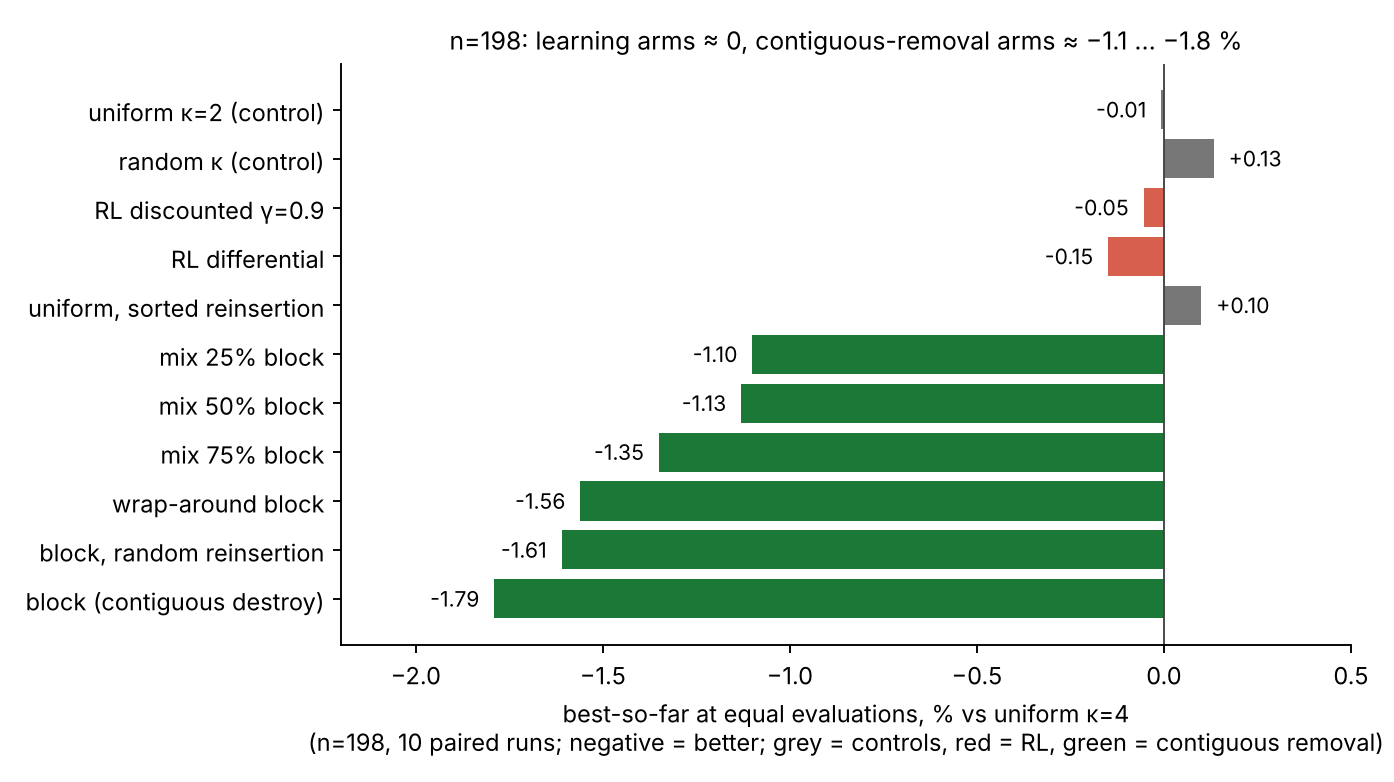
\includegraphics[width=0.95\textwidth]{Figures/fig8_attribution_n198.png}
\caption{Attribution at $n=198$ (10 paired runs), equal-evaluation best relative to uniform $\kappa=4$. Grey: controls; red: RL; green: arms removing contiguous groups. The gain grows with the share of contiguous removal.}
\label{fig:attribution}
\end{figure}

The idea of a \enquote{block} destroy was one of the four destroy-selection policies listed in stage R2 of the design brief, so the learning-based design is where the candidate entered the project, and the controlled-evaluation machinery built for it (equal-evaluation accounting, paired seeds, logged parent--offspring costs, pre-registered rules and control arms) is what allowed the effect to be found and verified. But no learned behaviour contributes to the gain: it is obtained by a fixed rule.

%----------------------------------------------------------------------------------------

\section{Why Learning the Destruction Size Did Not Help}\label{sec:discussion-why}

\begin{itemize}
\item \textbf{No headroom in $\kappa$.} At equal compute no $\kappa$ gives better final quality than another (Section~\ref{sec:exp-diag}). A learner can only exploit differences between actions; here the best constant is already optimal, and a constant is what the learner converges to.
\item \textbf{The cost, not the quality, differs.} A larger $\kappa$ costs proportionally more evaluations but produces mostly \emph{worse} offspring; the share of better offspring hardly changes. Hence the apparent advantage of small $\kappa$ in per-evaluation terms is a pure cost effect that a fixed $\kappa=2$ captures.
\item \textbf{Sparse, noisy reward.} Between 92\% and 98\% of offspring tie the parent and only about 1--3\% improve it (below 0.5\% late in the run). The average reward rate $\bar R$ is therefore near zero, changes sign dozens of times per run and gives the $-\bar R\tau$ term little structure to work with. This is the degeneration of the differential structure that the design brief itself warns about.
\item \textbf{Numerical fragility.} With the time unit in raw evaluations the coupled $Q$--$\bar R$ estimate diverged within about ten iterations; the stable version required a rescaling of the time unit.
\item \textbf{Discounting was not better.} The discounted variant was nominally the best RL arm on one instance but equal to the fixed $\kappa=2$ control within noise and did not replicate, so the claim that differential learning is superior to discounted learning is not supported by this data.
\end{itemize}

\section{Why a Fixed Operator Beats a Learned One Here}

A learner adds value when the best action \emph{changes with the search state}. For $\kappa$ no action is better than another at equal compute, so the optimum is a constant. For the destroy-selection operator, one action (contiguous removal) is better in every state that could be resolved at $n\ge198$, so a fixed choice already captures the whole gain; mixing the two operators was worse than using \texttt{block} alone, and no stagnation or budget cell favoured the uniform operator significantly. The only hint of state dependence (\texttt{block} better early, uniform better in the last quarter, at $n=400$ on one instance with five runs) is unconfirmed. A learner over operators would therefore have no resolvable signal to learn from at the sample sizes examined.

%----------------------------------------------------------------------------------------

\section{Comparison with the Expectations of the Design Brief}

\begin{table}[htbp]
\centering
\caption{Expectations stated in the design brief and the outcome.}
\label{tab:expectations}
\small
\begin{tabular}{P{4.4cm}P{8.6cm}}
\toprule
\textbf{Expectation} & \textbf{Outcome}\\
\midrule
RL controller gains $0.5$--$2\%$ at $n=200$, $1$--$3\%$ at $n=400$ & Gains of $1.97\%$ and $2.32\%$ were obtained, but by a fixed contiguous operator; the RL controller added $\approx0$\\
Little or no gain for $n\le50$ & Confirmed (mean change $0.00\%$)\\
Variance reduction is the more probable win & Not supported: run-to-run SD is about $9$--$12\%$ larger at $n\ge198$\\
\texttt{history-aware} destroy exploits the multi-predecessor structure (novelty claim) & Not supported at $n\le198$; $-0.29\%$ at $n=400$ is unproven\\
Differential RL outperforms discounted RL & Not demonstrated against the controls\\
An interpretable policy table characterises when large or small destruction pays off & Obtained, but it is trivial: $\kappa=2$ in every state\\
Learned shuffle removes the hand-tuned $\eta$ and $\delta$ constants & Not attempted (no state-dependent signal)\\
A negative result is publishable and should be planned for & Realised: learned destruction size is a controlled negative result\\
\bottomrule
\end{tabular}
\end{table}

%----------------------------------------------------------------------------------------

\section{Limitations and Threats to Validity}\label{sec:discussion-limits}

\begin{itemize}
\item \textbf{Baseline provenance.} The 60-instance comparison is against the published reference rows, reproduced exactly by our rebuild for 33 instances (all 31 with $n\le100$, one with $n=198$, one with $n=400$); the remaining 27 baseline rows were not re-run. The paired same-session design covers 10 instances (8 with $n\ge198$) and removes this dependence for them.
\item \textbf{Instance-level test.} The reference file contains only per-instance means, so the 60-instance test is over instances. Wilcoxon tests over the 26 large instances are as strong as the data allow ($p<0.0001$), but they cannot use run-level variation.
\item \textbf{Scope of the RL negative result.} Reduced protocol (10, 10 and 3 runs, one instance per size), online learning only, $\kappa$ as the only action, uniform destruction, no hyper-parameter sensitivity study. A learner over operators, a learned shuffle, offline training across an instance stream, and RL with \texttt{block} as the base operator were not tested. The nominal discounted-RL advantage at $n=100$ ($-1.10\%$) is unresolved.
\item \textbf{Scope of the \texttt{block} result.} Only $\kappa=4$ and uniform shuffle were tested in the full protocol. The mechanism is established only to \enquote{contiguity of the removed set}; the explanation through shared sensor history is a hypothesis.
\item \textbf{Exploratory statistics.} The experiments of Sections~\ref{sec:exp-diag}--\ref{sec:exp-mix} have uncorrected $p$-values, few runs at $n=400$ (five, so the smallest possible $p$ is $0.0625$) and about 25 contrasts per write-up. The full-protocol and same-session results do not rely on them.
\item \textbf{Paired design.} Pairing is by starting point only: the two arms use the same seeds, but the trajectories diverge. Within an instance the 20 runs are not independent of the instance, so pooled intervals resample instances and then runs; only four $n=400$ instances were in the paired subset, so that interval is narrower than a fresh-instance interval would be.
\item \textbf{Timing.} CPU times were measured with parallel jobs sharing the machine and are approximate.
\item \textbf{No GA comparison.} The previous method (GA-TRMP+LSB) was not re-run; its published figures are quoted for context only.
\end{itemize}

\section{Practical Implications}

For a practitioner the finding is simple and cheap: replace the uniform random choice of the destroyed groups in ES-TRMP by a contiguous block of the same size, for instances with at least about 200 groups. The change is one line of the destroy step, needs no learning phase, no additional parameters and no extra evaluations, and yields about $2\%$ lower total rotation (hence energy) at the sizes where the problem is hardest. For problems that share TRMP's structure of dependence on several predecessors, the same lesson applies more generally: before building an adaptive controller, test whether a fixed alternative operator dominates, because learning can only add value where the best choice varies with the state.
